\begin{framed}

Objetivos:
\begin{itemize}
    \item Entender por qué un perfil alar produce sustentación. 
\end{itemize}

Contenidos:
\begin{itemize}
    \item Repaso de superposición de flujos elementales para lograr un cilindro con sustentación.
    \item Flujos elementales con variable compleja. 
    \item La transformación de Joukowsky.
    \item La condición de Kutta.
    \item El vórtice de arranque.
\end{itemize}

Bibliografía:
\begin{itemize}
    \item White, F. M. (2008) Mecánica de Fluidos. McGraw-Hill. Sexta edición. Sección 8.4, 8.7.
    \item Batchelor, G. K. (2009) An Introduction to Fluid Mechanics. Cambridge University Press. Sección 6.7.
\end{itemize}
\end{framed}

\section*{Flujos elementales con variable compleja.}

En esta clase vamos a revisar una aplicación de flujo potencial: aerodinámica.
Hoy estudiaremos el flujo alrededor de perfiles alares, que son las responsables de que, por ejemplo, un avión se eleve.
Para esto, comenzaremos del análisis del flujo alrededor de un cilindro con sustentación, que estudiamos la clase pasada, y llegaremos a un perfil alar con una transformación topológica, lo que nos permitirá estudiar por qué un perfil alar produce sustentación con ecuaciones analíticas.

Antes de adentrarnos en aerodinámica como tal, nos conviene re-escribir las funciones de flujos elementales utilizando números complejos:
%
\begin{align}\label{eq:z_complejo}
z = x+iy\nonumber\\
\Phi = \phi + i\psi\nonumber\\
V = u+iv.
\end{align}

Usando las variables de la Ec. \eqref{eq:z_complejo}, podemos escribir los flujos elementales de manera equivalente a lo que ya conocemos:
%
\begin{itemize}
\item Flujo uniforme
%
\begin{align}\label{eq:flujo_uniforme_complejo}
\Phi_U &= U_\infty z\nonumber\\
       &= U_\infty (x+iy) = \phi_U + i\psi_U
\end{align}
%
\item Fuente
%
\begin{align}\label{eq:fuente_complejo}
\Phi_f &= \frac{q}{2\pi} \log(z)\nonumber\\
       &= \frac{q}{2\pi} \log\left(|z|e^{i\theta}\right) = \frac{q}{2\pi} \left(\log(r) + i\theta\right) = \phi_f + i\psi_f
\end{align}
%
\item Vórtice
%
\begin{align}\label{eq:vortice_complejo}
\Phi_v &= -i\frac{\Gamma}{2\pi} \log(z)\nonumber\\
       &= -i\frac{\Gamma}{2\pi} \log\left(|z|e^{i\theta}\right) = \frac{\Gamma}{2\pi} \left(i\log(r) - \theta\right) = \phi_v + i\psi_v
\end{align}
%
\item Doblete
%
\begin{align}\label{eq:doblete_complejo}
\Phi_d &= \frac{K}{z} \nonumber\\
       &= \frac{K\overline{z}}{z\overline{z}} = \frac{K}{|z|^2}(x-iy)\nonumber\\ 
       &= \frac{K}{r^2}(r\cos(\theta) - i\sin(\theta)) = \phi_d + i\psi_d
\end{align}

\end{itemize}

Usar esta formulación nos simplificará mucho la vida a la hora de operar sobre dobletes y vórtices que no están centrados en el origen, ya que solamente hay que reemplazar $z$ por $z-z_0$, donde $z_0$ es el centro del vórtice, doblete o fuente.
Es más, podemos generalizar las expresiones de flujo uniforme y doblete a considerar una inclinación de éstos. 
Para un ángulo de inclinación $\alpha$, el flujo uniforme nos queda:
%
\begin{equation} \label{eq:flujo_uniforme_complejo_angulo}
\Phi_U = U_\infty z e^{-i\alpha}
\end{equation}
%
y el doblete
\begin{equation} \label{eq:doblete_complejo_angulo}
\Phi_d = \frac{K}{z}e^{i\alpha} 
\end{equation}

Utilizando números complejos, podemos calcular $\phi$ y $\psi$ de un flujo que entra en un ángulo $\alpha$ alrededor de un cilindro centrado en $z_0$ con una sola ecuación:
%
\begin{align} \label{eq:cilindro}
\Phi_\text{cil} = \phi_\text{cil}+i\psi_\text{cil} = U_\infty z e^{-i\alpha} + \frac{K}{z-z_0}e^{i\alpha} -i\frac{\Gamma}{2\pi} \log(z-z_0).
\end{align}

Por ejemplo, un flujo entrante con velocidad $U_\infty=1$ y $\alpha=8^\circ$ que pasa alrededor de un cilindro con radio $r=1.1$, centrado en $(-0.1,0)$ y con circulación $\Gamma=-1$ tiene las líneas de flujo de la Figura \ref{fig:flujo_cil} y las líneas de equipotencial de la Figura \ref{fig:phi_cil}
%
\begin{figure}[h!]
\centering
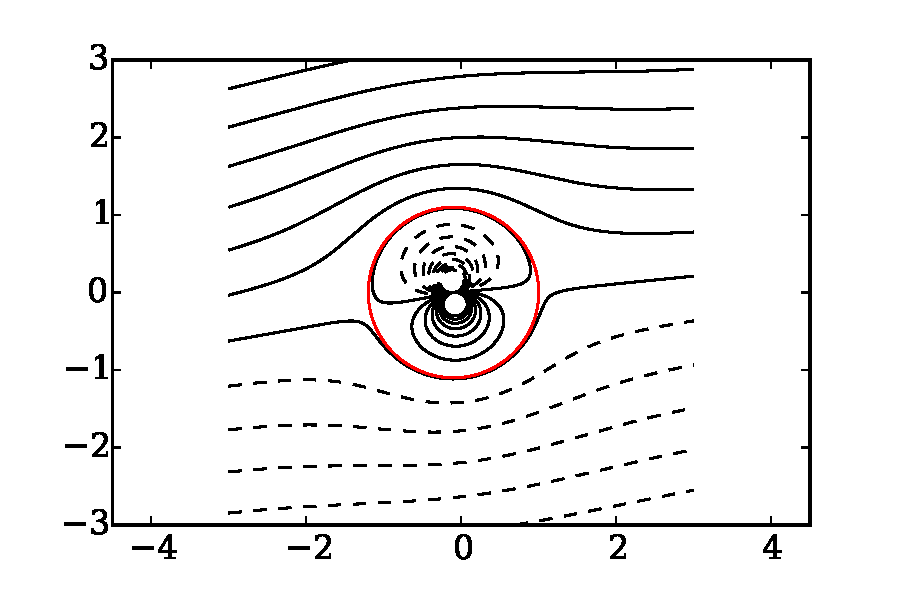
\includegraphics[width=0.7\textwidth]{clase05/flujo_cil.pdf}
\caption{Líneas de flujo a $U_\infty=1$ y $\alpha=8^\circ$ alrededor de cilindro $r=1.1$ centrado en $(-0.1,0)$ con circulación $\Gamma=-1$}\label{fig:flujo_cil}
\end{figure}
%
\begin{figure}[h!]
\centering
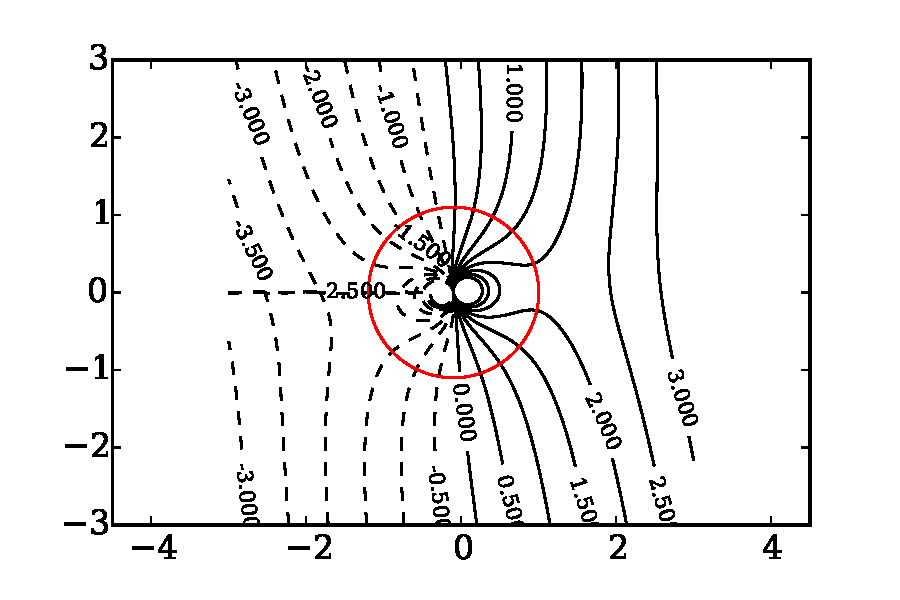
\includegraphics[width=0.7\textwidth]{clase05/phi_cil.pdf}
\caption{Líneas de equipotencial a $U_\infty=1$ y $\alpha=8^\circ$ alrededor de cilindro $r=1.1$ centrado en $(-0.1,0)$ con circulación $\Gamma=1$}\label{fig:phi_cil}
\end{figure}

Para calcular la fuerza del doblete ($K$) usamos el radio del cilindro, que de la clase anterior sabemos que es $r=\sqrt{K/U_\infty}$.

\section*{Transformación de Joukowsky}

La transformación de Joukowsky nos permite mapear un círculo a un perfil aerodinámico. 
Si $\zeta = \xi + i\eta$ son los puntos de un círculo en el plano $\zeta$, la tranformación de Joukowsky es
%
\begin{equation}
z = \zeta + \frac{k^2}{\zeta}
\end{equation}
%
donde $z=x+iy$ son los puntos que definen el perfil aerodinámico, y $k$ es un factor que define el tamaño ($k\approx4c$, donde $c$ es la cuerda del perfil). 
Eso si, existe una condición: el contorno del círculo debe intersectar el punto $\xi=k, \eta=0$, y el punto $\xi=-k, \eta=0$ debe estar contenido dentro del círculo. 
Esto es porque un perfil aerodinámico tiene un lado puntiagudo atrás (cúspide), los cuales son reproducidos por los puntos singulares de la transformación (donde la derivada de la transformación es cero); esto ocurre en $\xi=k, \eta=0$ y $\xi=-k, \eta=0$.
De hecho, si el círculo está centrado e intersecta los dos puntos críticos, la transformación entrega una línea (Figura \ref{fig:perfil_linea}), que es la única forma de tener dos cúspides.
Por lo tanto, de no cumplir estas condiciones, la transformación genera geometrías que no se asemejan a un perfil aerodinámico.

\begin{figure}[h!]
\centering
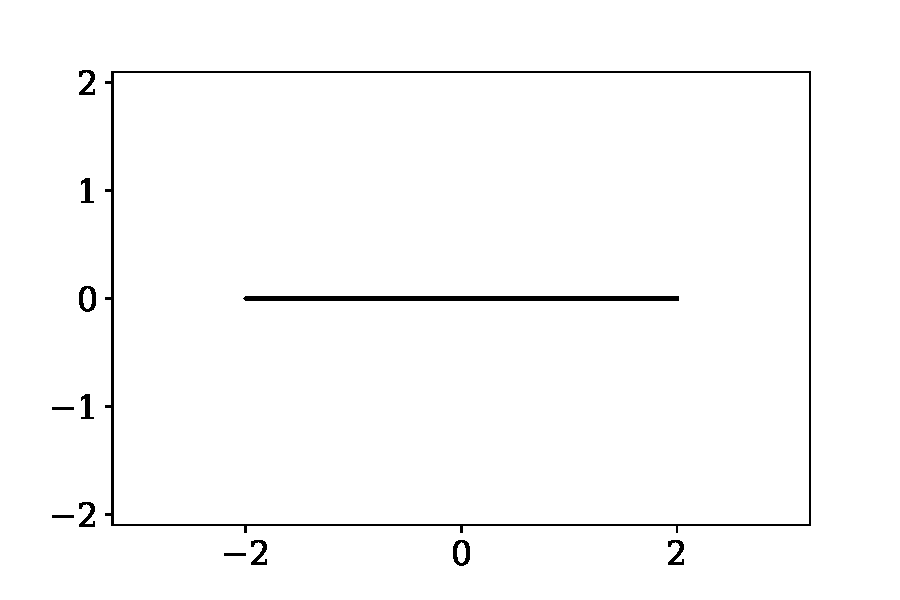
\includegraphics[width=0.7\textwidth]{clase05/perfil_linea.pdf}
\caption{Resultado de transformación de Joukousky a cilindro centrado en el origen, con $k=1$}\label{fig:perfil_linea}
\end{figure}


La Figura \ref{fig:perfil_simetrico} muestra la tranformación de Joukouwsky sobre un círculo centrado en $\xi=-0.1, \eta=0$, con $k=1$).
Como ven, se genera un perfil aerodinámico simétrico.
%
\begin{figure}[h!]
\centering
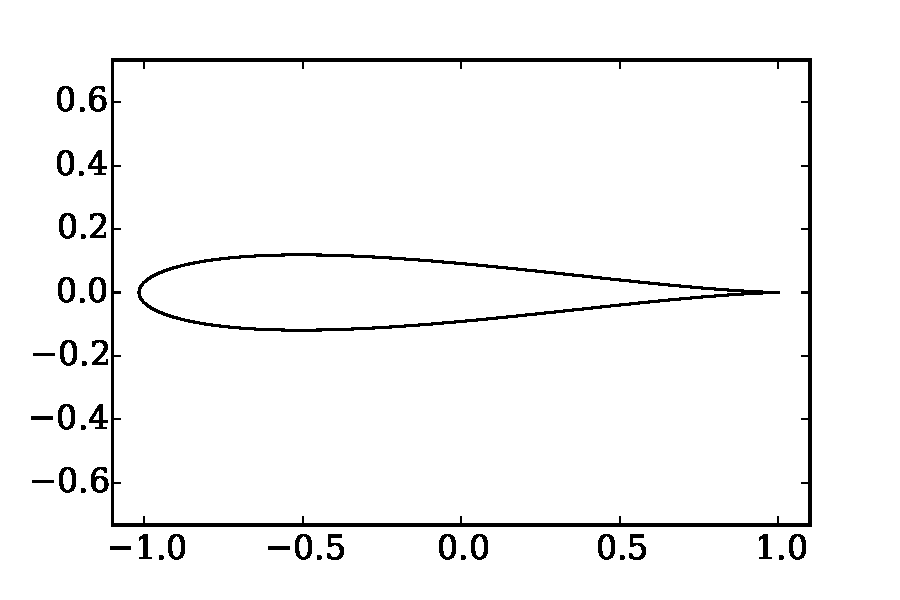
\includegraphics[width=0.7\textwidth]{clase05/perfil_simetrico.pdf}
\caption{Resultado de transformación de Joukousky a cilindro centrado en $\xi=-0.1, \eta=0$}\label{fig:perfil_simetrico}
\end{figure}
%
Podemos así jugar con la posición del cilindro para variar la geometría del perfil, donde la posición $\xi$ del centro modifica el ancho del perfil, y $\eta$ la curvatura.
Por ejemplo, la Figura \ref{fig:perfil_simetrico_ancho} es el resultado de la transformación de un cilindro centrado en $\xi=-0.2, \eta=0$, y como ven, es mucho más ancho que la Figura \ref{fig:perfil_simetrico}.
%
\begin{figure}[h!]
\centering
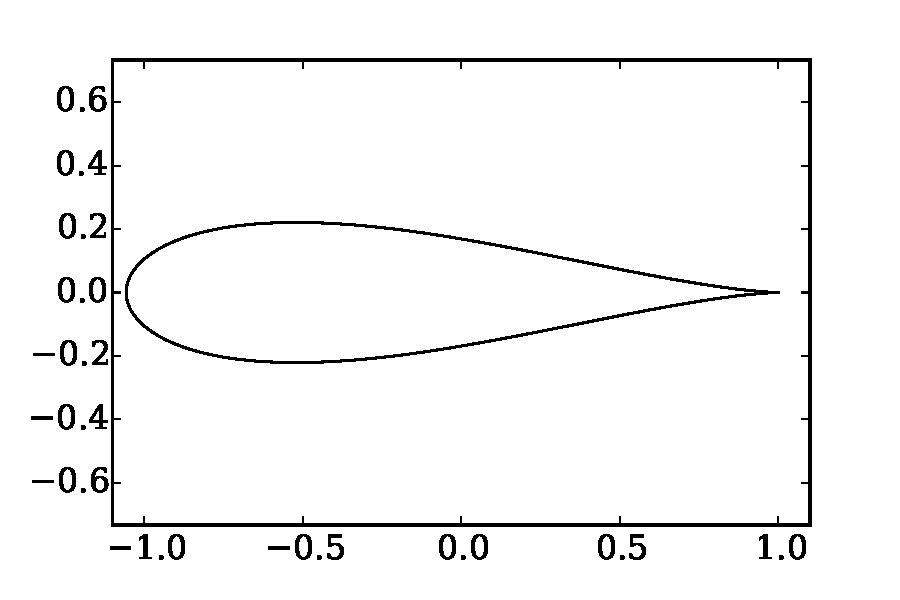
\includegraphics[width=0.7\textwidth]{clase05/perfil_simetrico_ancho.pdf}
\caption{Resultado de transformación de Joukousky a cilindro centrado en $\xi=-0.2, \eta=0$, y $k=1$}\label{fig:perfil_simetrico_ancho}
\end{figure}

Por otra parte, la Figura \ref{fig:perfil_curvo} resulta de aplicar la transformación a un círculo centrado en $\xi=-0.1, \eta=0.1$, ejemplificando que de mover el centro en el eje $\eta$ el perfil toma una curvatura.
%
\begin{figure}[h!]
\centering
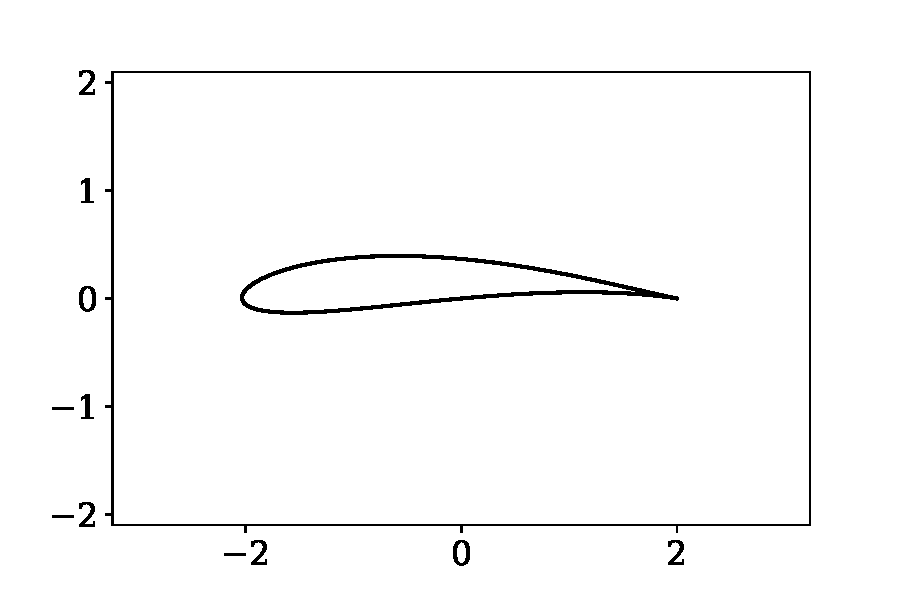
\includegraphics[width=0.7\textwidth]{clase05/perfil_curvo.pdf}
\caption{Resultado de transformación de Joukousky a cilindro centrado en $\xi=-0.1, \eta=0.1$, con $k=1$}\label{fig:perfil_curvo}
\end{figure}

\section*{Flujo alrededor de un perfil alar y la condición de Kutta}

Utilicemos la transformación de Joukowsky para estudiar el flujo alrededor de un perfil alar.
El caso más simple es el cilindro sin circulación, y un flujo de entrada sin ángulo.
Si centramos el cilindro en el punto $(-0.1,0)$ (el radio es tal que el círculo intersecta el punto $(1,0)$) y el flujo de entrada tiene $U_\infty=1$, obtenemos el flujo de la primera imagen de la Figura \ref{fig:flujo_cil_simple}, y si a eso le aplicamos la transformación de Joukowsky, obtenemos el flujo al rededor del perfil de la misma figura.
%
\begin{figure}[h!]
\centering
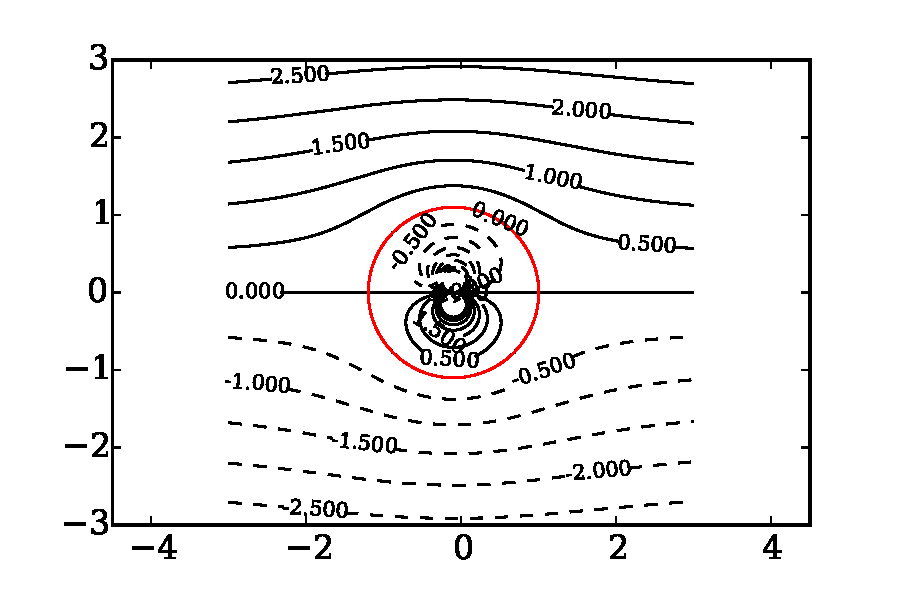
\includegraphics[width=0.7\textwidth]{clase05/flujo_cil_simple.pdf}
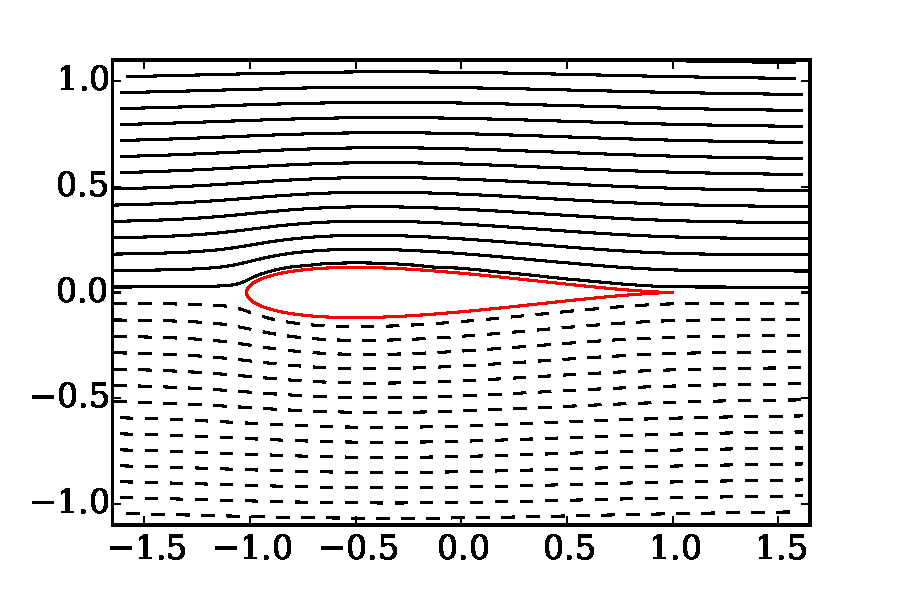
\includegraphics[width=0.7\textwidth]{clase05/flujo_perfil.pdf}
\caption{Flujo alrededor de perfil alar que resulta de la transformación de un cilindro centrado en $\xi=-0.1, \eta=0.$ con un flujo entrante de $U_\infty=1$.}\label{fig:flujo_cil_simple}
\end{figure}

El flujo de la Figura \ref{fig:flujo_cil_simple} se comporta como esperamos, pero no es muy interesante.
En aplicaciones reales, las alas de los aviones se enfrentan al flujo en un ángulo (el ángulo de ataque).
Podemos agregar este efecto a través de $\alpha$ en la Ec. \eqref{eq:cilindro}.
A modo de ejemplo, si en el flujo en la Figura \ref{fig:flujo_cil_simple} consideramos $\alpha=15^\circ$, llegamos a la Figura \ref{fig:flujo_perfil_alpha15} 
%
\begin{figure}[h!]
\centering
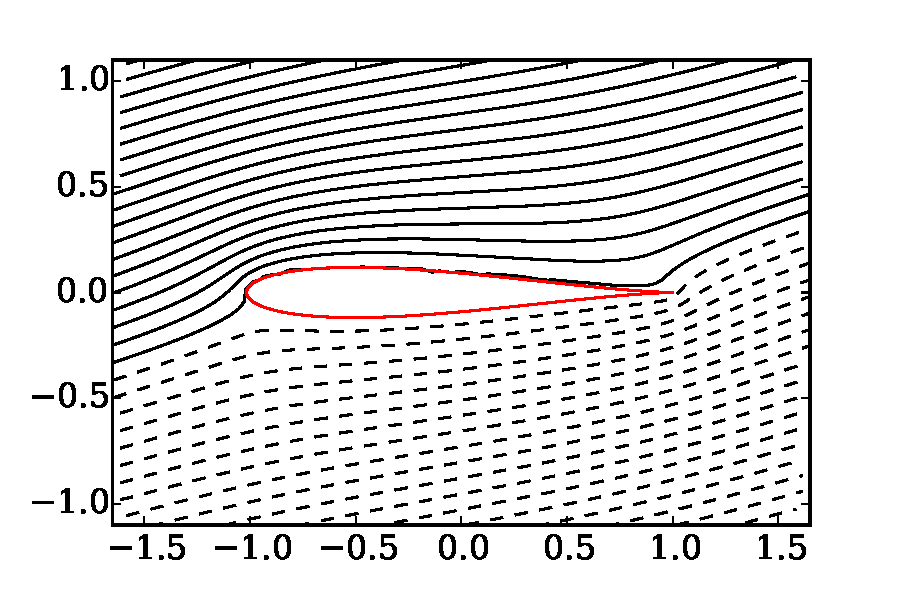
\includegraphics[width=0.7\textwidth]{clase05/flujo_perfil_alpha15.pdf}
\caption{Flujo alrededor de perfil alar que resulta de la transformación de un cilindro centrado en $\xi=-0.1, \eta=0.$ y un flujo entrante de $U_\infty=1$ y ángulo de ataque $\alpha=15^\circ$.}\label{fig:flujo_perfil_alpha15}
\end{figure}

La Figura \ref{fig:flujo_perfil_alpha15} tiene algo raro: el flujo en la parte de atrás se escapa del perfil alar en un ángulo diferente al del perfil, lo que no tiene mucho sentido físico.
Si uno revisa imágenes del flujo detrás de perfiles alares\footnote{\url{https://www.youtube.com/watch?v=6UlsArvbTeo}}, se da cuenta que el perfil alar desvía al flujo, y sale tangencial a la punta posterior.
Es más, en la figura \ref{fig:flujo_perfil_alpha15} da la impresión que las líneas de flujo de la parte inmediatamente inferior al perfil alar están curvándose hacia arriba y ``devolviéndose'' aguas arriba por la parte superior, lo cual es algo que la viscosidad no permite hacer.
Sabemos que la viscosidad tiene que ver con el ``arrastre'' que un elemento de fluido produce en su vecino, y se podrán imaginar que si un elemento de fluido es arrastrado por sus vecinos, este no puede doblar por una esquina tan pronunciada.
A pesar que nuestro modelo es no viscoso, por lo que genera este tipo de resultados no físicos, debemos hacernos cargo de alguna forma de este efecto viscoso.

Hasta ahora, no hemos considerado una circulación; agreguémosla a nuestro modelo.
Si consideramos $\Gamma=-2$ (negativo pues el vórtice debe rotar en sentido horario) en el flujo de la Figura \ref{fig:flujo_perfil_alpha15}, obtenemos el flujo de la Figura \ref{fig:flujo_perfil_gamma2}
%
\begin{figure}[h!]
\centering
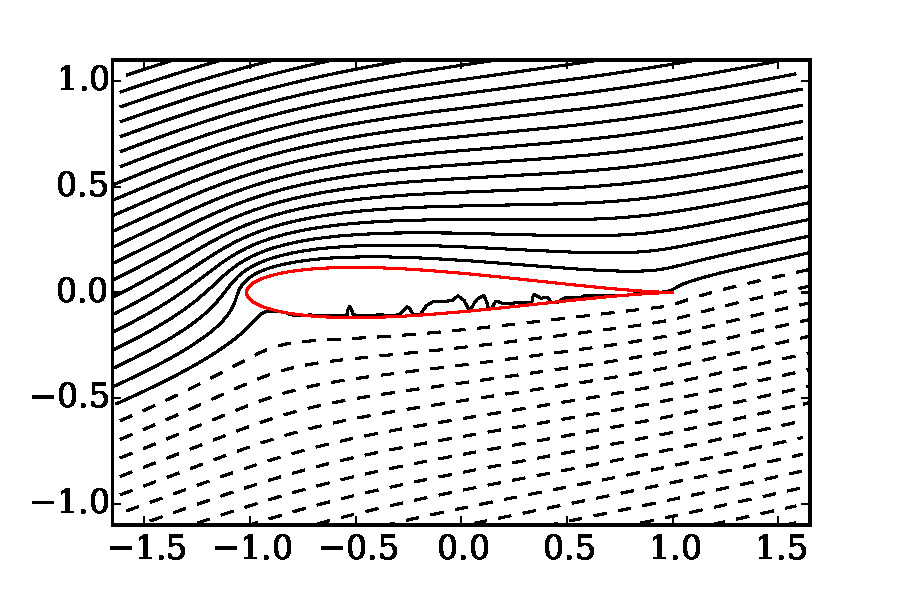
\includegraphics[width=0.7\textwidth]{clase05/flujo_perfil_gamma2.pdf}
\caption{Flujo alrededor de perfil alar que resulta de la transformación de un cilindro centrado en $\xi=-0.1, \eta=0.$ con $\Gamma=-2$ y un flujo entrante de $U_\infty=1$ y ángulo de ataque $\alpha=15^\circ$.}\label{fig:flujo_perfil_gamma2}
\end{figure}

La Figura \ref{fig:flujo_perfil_gamma2} parece mejorar con respecto a \ref{fig:flujo_perfil_alpha15}, ya que las líneas se acercan a ser tangentes al perfil alar, pero todavía no lo son.
Probemos con $\Gamma=-5$, como lo muestra la Figura \ref{fig:flujo_perfil_gamma5}.
%
\begin{figure}[h!]
\centering
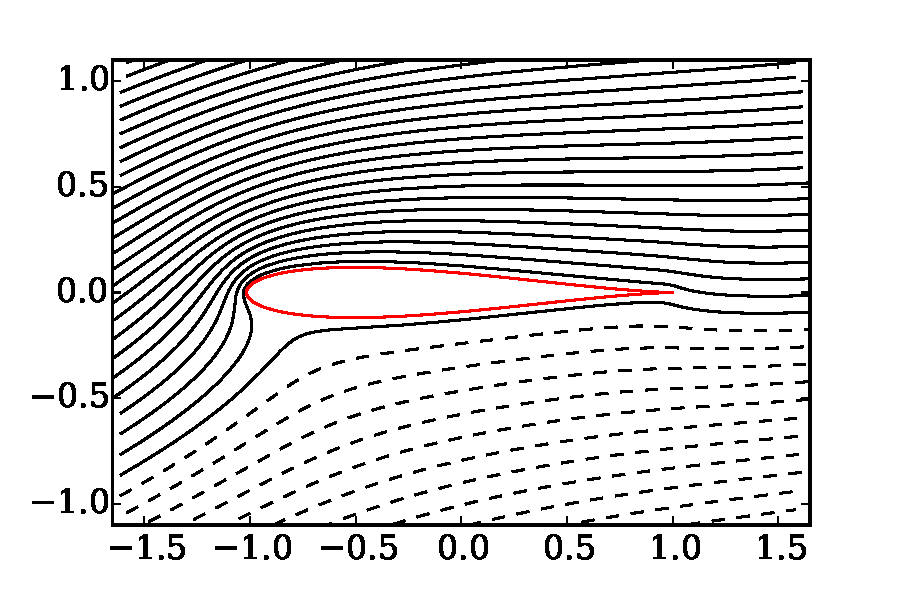
\includegraphics[width=0.7\textwidth]{clase05/flujo_perfil_gamma5.pdf}
\caption{Flujo alrededor de perfil alar que resulta de la transformación de un cilindro centrado en $\xi=-0.1, \eta=0.$ con $\Gamma=-5$ y un flujo entrante de $U_\infty=1$ y ángulo de ataque $\alpha=15^\circ$.}\label{fig:flujo_perfil_gamma5}
\end{figure}

En el caso de la Figura \ref{fig:flujo_perfil_gamma5} nos hemos pasado con mucha circulación , ya que las líneas de flujo aparecen apuntando hacia abajo.

Intentémoslo con $\Gamma=-3.6$.
Este resultado corresponde a la Figura \ref{fig:flujo_perfil_gamma3}, y parece ser que el flujo sale perfectamente tangencial al perfil alar.
%
\begin{figure}[h!]
\centering
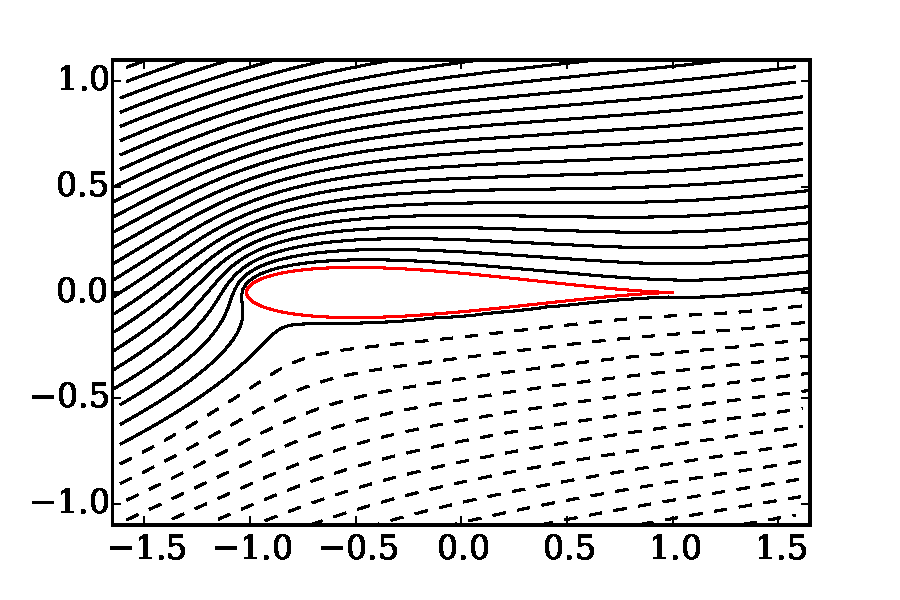
\includegraphics[width=0.7\textwidth]{clase05/flujo_perfil_gamma3.pdf}
\caption{Flujo alrededor de perfil alar que resulta de la transformación de un cilindro centrado en $\xi=-0.1, \eta=0.$ con $\Gamma=-3.6$ y un flujo entrante de $U_\infty=1$ y ángulo de ataque $\alpha=15^\circ$.}\label{fig:flujo_perfil_gamma3}
\end{figure}

El resultado de la Figura \ref{fig:flujo_perfil_gamma3} es el físicamente correcto.
A pesar de que todas las pruebas que hicimos acá cumplen con el flujo potencial, solamente una de ellas tiene relevancia física, pues se hace cargo del efecto de la viscosidad.
Esta condición de tangencialidad a la salida del perfil alar se conoce como \emph{condición de Kutta}.

\section*{La condición de Kutta y sustentación}

En palabras más técnicas, la condición de Kutta dice que un cuerpo con un lado puntiagudo genera la cantidad de circulación al rededor de si mismo necesario para mantener un punto de estancamiento en la punta.
Esto tiene trementa implicancia en la física, y empezamos a responder la pregunta \mbox{?`}Por qué vuelan los aviones?
La gracia de que trabajamos con el perfil de Joukowsky es que se hace patente que al estar en un ángulo genera sustentación, pues es equivalente a un cilindro con sustentación.
Si $\Gamma_\text{Kutta}$ es la circulación que cumple con la condición de Kutta (para que la solución tenga relevancia física), la fuerza sobre el perfil alar es
%
\begin{equation}
L = \rho\Gamma_\text{Kutta}U_\infty,
\end{equation}
%
que es la sustentación sobre el cilindro equivalente.

En resumen \mbox{?`}por qué un ala es capaz de levantar un avión? Por que el ángulo del ala desvía el flujo hacia abajo y la punta de la parte posterior del perfil alar fuerza al flujo a salir tangencial (por viscosidad).
Esto genera una circulación alrededor del ala que resulta en una fuerza de sustentación.
El flujo potencial no es capaz de reproducir esto por si solo, ya que no considera viscosidad, y debemos agregarle al flujo una circulación $\Gamma_\text{Kutta}$ tal que se cumple la condición de Kutta.

El que exista una transformación analítica que nos lleve a un perfil aerodinámico es un caso muy particular de los perfiles de Joukousky, pero no es el caso general. 
Por lo tanto, para un perfil sin una transformación hay que monitorear la velocidad a la salida del perfil para ver si hay estancamiento, y así encontrar $\Gamma_\text{Kutta}$.

Para Joukowsky, podemos aprovechar que si existe una transformación para calcular analíticamente $\Gamma_\text{Kutta}$. 
Sabemos que el punto del cilindro que mapea a la punta es el punto singular $(1,0)$, por lo tanto, la condición de Kutta se cumple tal que el punto de estancamiento en el cilindro se encuentre en $(1,0)$ en el cilindro.

Usando variable compleja, la función potencial en el caso del cilindro esta dado por Ec. \eqref{eq:cilindro}, y la velocidad es
%
\begin{equation}
V = u+iv = \frac{d\Phi_\text{cil}}{dz} = U_\infty e^{-i\alpha} - \frac{K}{(z-z_0)^2}e^{i\alpha} - i\frac{\Gamma}{2\pi(z-z_0)}.
\end{equation}
%
Sabiendo que $R = \sqrt{K/U_\infty}$, y que en el punto de estancamiento $V(1,0)=0$, podemos despejar $\Gamma_K$
%
\begin{equation}
\Gamma_\text{Kutta} = -2\pi i\left[ U_\infty e^{-i\alpha}(z-z_0) - \frac{R^2U_\infty}{z-z_0}e^{i\alpha}\right]
\end{equation}

\subsection*{Vórtice de arranque}
Hace un par de clases discutimos algo que quizás pasó algo desapercibido, pero hoy lo revisitamos: el teorema de circulación de Kelvin
%
\begin{equation}
\frac{D\Gamma}{Dt}=0
\end{equation}

El teorema de circulación de Kelvin dice que para un flujo no viscoso, la circulación se mantiene constante en el tiempo.
La solución que aparece graficada en la Figura \ref{fig:flujo_perfil_gamma3} no es más que el estado estacionario de un problema transiente, que tiene que haber partido con velocidad cero.
Aquí salta algo extraño: si el flujo está quieto, $\Gamma=0$, sin embargo, en el estado estacionario $\Gamma=\Gamma_\text{Kutta}$, por lo que se generó circulación de alguna manera y aparentemente estamos violando el teorema de circulación de Kelvin.
Resulta que cuando el flujo inicia su movimiento, se desprende del perfil alar un vórtice con exactamente la circulación contraria $\Gamma=-\Gamma_\text{Kutta}$, que se conoce como \emph{vórtice de arranque}, cancelando la circulación total.
El vórtice de arranque se puede ver en simulaciones\footnote{\url{https://www.youtube.com/watch?v=B-tcx5hTf_A}} y con experimentos muy simples.\footnote{\url{https://www.youtube.com/watch?v=t7Sp4Nd9cg0}}

La circulación se define como
%
\begin{equation}
\Gamma = \oint_L\mathbf{V}\cdot\mathbf{t}dl,
\end{equation}
%
donde $L$ es una curva cerrada, de la cual el vector $\mathbf{t}$ es tangente, y $dl$ es un elemento de $L$.
Si $L$ es una curva que encierra al perfil alar solamente, inicialmente calcularíamos $\Gamma=0$, y en el estado estacionario $\Gamma=\Gamma_\text{Kutta}$.
Sin embargo, si $L$ encierra tanto el perfil alar como el vórtice de arranque (que probablemente está lejos aguas abajo), $\Gamma=0$ y se cumple el teorema de la circulación de Kelvin.
